\chapter{Background \& Objectives}

% This section should discuss your preparation for the project, including background reading, your analysis of the problem and the process or method you have followed to help structure your work.  It is likely that you will reuse part of your outline project specification, but at this point in the project you should have more to talk about. 
% 
% \textbf{Note}: 
% 
% \begin{itemize}
%    \item All of the sections and text in this example are for illustration purposes. The main Chapters are a good starting point, but the content and actual sections that you include are likely to be different.
%    
%    \item Look at the document on the Structure of the Final Report for additional guidance. 
%    
% \end{itemize}

\section{Background}
Researchers at Aberystwyth University have been studying three species of yeast, \textit{Candida tropicalis}, \textit{Candida boidinii}, and \textit{Candida shehatae}. To study the genetics of these species, they have each had their genomes sequenced by Illumina sequencing machines. From that point the sequences of DNA that have been read are then assembled into contigs (contiguous DNA fragments). This process produces an accurate representation of the species DNA, which then can then be aligned to other better understood DNA and annotated as such.

Arabinose and Xylose are five carbon sugars ubiquitously found in plants such as grass, which can be used as a feedstock for industrial biotechnology. \textit{Candida tropicalis} is able to convert arabinose \& xylose into arabitol and xylitol respectively. Xylitol is a commercially valuable anti-bacterial food grade sugar use in the manufacture of chewing gum. However arabitol and xylitol are stereo isomers and cannot be easily separated. \textit{Candida boidinii} cannot metabolise arabinose, for an unknown reason, but does metabolise Xylose but at a much slower rate which is commercially in-viable.

Understanding at a genomic level why \textit{Candida boidinii} is unable to utilise arabinose and genetically modifying \textit{Candida tropicalis} to have the same phenotype, may enable \textit{Candida topicalis} to exclusively produce xylitol and not arabitol. This would mean a cheap and easy way to produce a source of Xylitol, which can be used for many applications. One exciting possibility is using it as a low glycaemic index table sugar that can be used by diabetics.

Currently the researchers have the genetic information for the three species of yeast in their raw data format, a fasta file. These files are large \textgreater 16MB text files that are quite difficult to navigate and manipulate for less technically minded biologists. To make predictions about what genes perform what functions in the yeasts they will need to be able to search and browse this data in a much easier to interact with form. 

This is why a website would be advantageous to them, as it would provide a simple and familiar user experience to other web based genome browsers such as the Candida Genome Database\cite{cgd}. In addition to this functionality, one task that would be very useful is to be able to select a proteins coding sequence of nucleotides and then a user defined number of bases up and down stream of the gene, so that when they test out a theory in the wet lab experiments they can easily retrieve the bases around the gene that they intend to modify. 

\section{Existing Databases}
As the core of the project focuses on having the data ingested into a database, the first action was to investigate the current database solutions that had been developed for genomic information. 

The most well established was CHADO\cite{chado} which was initially developed back in 2005 for the FlyBase\cite{flybase} project. It has since then grown to accommodate genomic information for eukaryotes, plants, and other complex multicell animals. It uses PostgreSQL\cite{postgres} to store it's data and Perl\cite{perl} to setup and maintain the database. Due to it's monolithic approach of being a one size fits all solution, it has over 200 tables in a very complex schema. This makes working on it rather difficult, as there are many relations to consider when entering and manipulating data from the database.

When installing and populating CHADO, it was clear that the project wasn't very well maintained as during the installation several of the Perl modules that it depends on where failing their tests and not installing. This meant several modules had to be manually fixed just to get the application to install correctly. If it takes an experienced programmer and Linux admin several hours to follow the default installation instructions, debugging issues at several steps, it isn't going to be appropriate to impose such a system on potentially less technically minded Biologists. This combined with the fact that Perl has now been superseded by more modern scripting languages such as Python\cite{python} and JavaScript\cite{node}, thanks to their superior package management, eco-systems and syntax, it was clear that a more modern approach would be more sustainable and maintainable for this project and for the future. 

\section{Alignment Tools}
As the source of the data was uncertain, it was decided to investigate performing alignments in the event that more data, or different data was needed for the project than what was provided. The original alignment tool BLAST\cite{blast} was developed in the 90's and is very widely accepted as the de facto standard for performing alignments. 

Alignment is when a DNA, or protein sequence is compared against a database of known protein sequences that have already been determined via previous research. This allows a researcher to match their sequences against known proteins and annotate them accordingly. These annotations aren't proof that the gene codes for that exact protein, but it is a strong indicator that it does. To prove it the researchers will test it in a lab experiment, however as there are many thousands of potential genes to test it is a lot more efficient to test genes that are predicted via an alignment. 

An alignment is a computationally intensive task there have been many efforts to improve the efficiency of the algorithm and make the most of developments made in computing since the 90's. One area that has been pursued is the use of GPU's to perform alignments in parallel utilising hundreds or thousands of cores of the GPU, compared to the tens of cores on a modern CPU. 

Initially Diamond\cite{diamond} was tested and was able to align the data sets against the NCBI\cite{ncbi} non-redundant protein database\cite{nr}, in about an hour and a quarter for each species, this was only using the CPU and may have been bottlenecked by the mechanical drives being used as storage. 

The hardware being used for this was an Intel i7-6700k @ 4.6Ghz, 16GB of RAM, a 7200rpm Hard Disk Drive, and a Nvidia GTX 980. 

As there was a high performace graphics card available it would be advantageous to make use a GPU accelerated alignment tool to make the most of the hardware available, and reduce the time that any future alignments may take. 

The first attempt to use a GPU powered tool was BarraCUDA\cite{barracuda}, which installed successfully and appeared to run fine, however it would attempt to read in the entire reference database into memory. This was an issue as the NCBI non-redundant database is around 66GB in size, and the system that was being used only had 16GB of RAM available. 

The next tool tested was CLAST\cite{clast}, which unfortunately had compilation errors on the system. Debugging this was out of scope for my project as in this initial stage it didn't seem necessary. Next tested was Cudasw++\cite{cudasw} this did install, but ran into the same issues as Barracuda, being limited by the system memory available. 

In an attempt to get GPU acceleration working, the NCBI nr database was split up into 10GB chunks for use with these tools, however even after being reduced in size, BarraCUDA and Cudasw++ both had errors and failed to complete an alignment. 

It was decided that although the speed gains of a GPU accelerated alignment tool would be significant, the Diamond alignment was quick enough to not be a major bottleneck for the project, when compared with the extra time and effort that would have to be put into investigating how to get the GPU alignments to work. 

\section{Differences in Bioinformatics and Computer Science}
From studying bioinformatics and researching the most common methods of manipulating and analysing the data gathered, a trend was in the solutions being used was observed. 

In computer science, tools are highly developed and have evolved to a very stable state and the best tools are known to be industry standards for their specialised purposes. 

However in bioinformatics a combination of factors including the relative youth of the field and the large number of competing projects that don't collaborate due to competing for research publications; there have been a wide array of tools created, often by biologists with no software engineering experience, none of which have been adopted and honed as the de facto standard. 

This means that for every task in the bioinformatics space there is often many different solutions offered, to what can be a very simple problem. An example of this is the simple task of splitting a fasta file up into several chunks, this should be a very simple problemto solve, and once it's been solved once that tool should become the one tool to complete that task. 

Unfortunately when trying to do this, several tools were discussed on biostars forum\cite{biostars}, none of which worked for the nr database that was trying to be split. Eventually a tool made by Gordon Gremme et al\cite{genometools} was able to complete the task, yet it wasn't mentioned in the earlier discussion on the online forum. 

As a computer scientist this is a very odd observation, as for most problems in the programming sphere will have had several tools developed to solve it. The community then quite quickly picks the best solutions and adopts them as the known standards.\cite{needed}. 

An example of this is data markup languages, there are really only three major competing standards, XML, JSON and YAML, and they each have their own niche. However in bioinformatics there seems to be many ways to represent data from alignments or sequences. Fasta is appearing to be the most mature way however there are so many standards, tab separated, gff3, EMBL and SAM files to name a few. 

It seems very misguided to have produced all these new file formats, instead of a standard mark up language to represent the data. Fasta could very easily be replace by YAML, which would save a huge amount of developer time as they wouldn't have to produce or implement a fasta parser in their language of choice, as YAML can be natively read by most modern languages. 

%\subsection{My motivation}
%% What was your motivation and interest in this project?  
%
%My interest in this project stems from my interest in genetics, something that has always fascinated me since I learned about how we evolved into being. As a computer scientist I relish the chance to apply the knowledge of my domain, to a real life application that can have a measurable positive impact on the world. Hopefully I will be able to use this experience to further my career into bioinformatics as well as helping contribute to the research being done. 

\section{Analysis}
% Taking into account the problem and what you learned from the background work, what was your analysis of the problem? 

From researching the current solutions to the problem of annotating, storing and presenting genetic information, it was clear that a solution using modern web development technologies wasn't currently in the public or open source domain. 

Of the open source projects that were currently in use the majority appeared to be very old and monolithic. This is often due to their integration with the most popular genome viewers GBrowse\cite{gbrowse} and JBrowse\cite{jbrowse} which are both written in Perl.

Perl is not suited to modern web development, mainly due to it's miniscule market share\cite{perl-market} and vastly smaller number of available third party modules. 

\begin{figure}[ht!]
\begin{center}
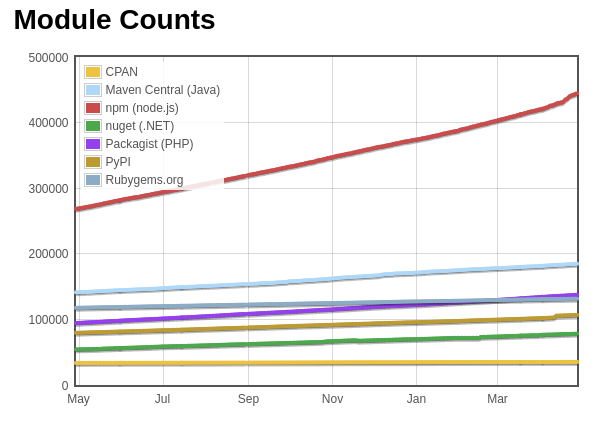
\includegraphics[scale=0.7]{module-count}
\caption{Number of modules available for server side languages, Perl (CPAN), Java (Maven), JavaScript (npm), .NET (nuget) PHP (Packagist), Python (PyPI), Ruby (Gems)\cite{modulecounts}}
\end{center}
\end{figure}

Web development simply isn't done in Perl any more, and that means that the ecosystem surrounding it just can't compete with newer technologies such as Ruby on Rails or Node JS.

\subsection{Analysis of the problem}
Looking at the data that I was provided with there was three clear stages to the development of my solution. The first would be to ensure that the data I had was valid and in the same format for each of the species that were being analysed. The next was to import that data into a database, and then from there develop a web front end to interact with the data in the database. 

An alternative approach to this project would be to use one of the existing databases such as Intermine\cite{intermine} or CHADO\cite{chado}, and then use a web front end compatible with those databases such as GBrowse\cite{gbrowse} or Jbrowse\cite{jbrowse}. This would require slight changes to how the data was processed before going into these established systems, however the benefit of using this approach would be access toa ll of the bioinformatics tools that are compatible with these platforms.

As a computer scientist looking at this problem, there doesn't seem to be much need for a very complex solution. Once the data is generated, the hard bit, it just needs to be made into a database friendly format and then ingested to the database system. From there building a simple web front end to make the database accessible is a very simple task. There isn't any need to manipulate or modify the data, simply create and read it. Because of this it seemed that the current systems were greatly over complicating matters.

  \subsection{SQL vs NoSQL databases}

  Structured Query Language (SQL) databases such as MariaDB, PostrgeSQL and SQLite, store data in a relational manner, this means that data is stored across many linked tables, that are grouped by the data type. They are the interfaced with via SQL to select related data from multiple tables to return a meaningful result. 
  
  \begin{itemize}
    \item SQL based systems have been used for a long time and have a large amount of support and compatibility with different frameworks. 
    \item Efficient storage of data, not duplicated
    \item Complex queries can be ran with relative ease
    \item Requires a strict schema 
    \item Development is more complex as you have to manage and maintain relations
  \end{itemize}

  NoSQL databases store data in collections of documents. Each collection is usually linked to a use case for the data, for example a website that has blog posts would have a "blog" collection, that stores all of the data for blog posts. The collection is made up of indivdual documents representing individual items, so the "blog" collection will store lots of individual blog posts. Each document is then made up of key value pairs, commonly represented as JSON. 

  \begin{itemize}
    \item Collections are based on use cases so no complex selection logic
    \item Data is represented as JSON so it is very interoperable with JavaScript
    \item Dynamic schema, not every document has to have the same information as the other documents in the collection
    \item Newer technology so less legacy support
    \item Data can be stored twice which is less efficient
  \end{itemize}

% There should be a clear statement of the research questions, which you will evaluate at the end of the work. 

% In most cases, the agreed objectives or requirements will be the result of a compromise between what would ideally have been produced and what was felt to be possible in the time available. A discussion of the process of arriving at the final list is usually appropriate.

\section{Research Method and Software Process}
It was intended to use a blend of agile and extreme programming methodologies for this project. The idea was to ensure that as the understanding of the task at hand increased and new requirements or changes to the structure of the application became necessary, an agile workflow would allow adaptations to be made without setting the project's progress back. 

For this project there were clear clients that could be accessed and used for feedback during development iterations. David Bryant and Abhishek Somani, the scientists conducting the research were available to meet and provide feed back. When suitable we would meet on a Friday at the end of an iteration to discuss the projects progress and any difficulties that may have been encountered. Towards the end of the project this time was used to get detailed feedback on how the website could be improved. 

Unit testing was also used to develop the key algorithms, as well as continuous integration and deployment, this process is described in much more detail later on in the document. It was key to being able to deliver working software at regular intervals and demonstrate it to the clients. 

Once requirements were gathered a Kanban board would be made with each individual task listed, based on the requirements of the application. Those tasks would then be weighted with an estimated difficulty, and then worked on. Once development had started on each task it would be moved to the "In progress" board, and then across to the "Done" board, once completed. 

\begin{figure}[ht!]
\begin{center}
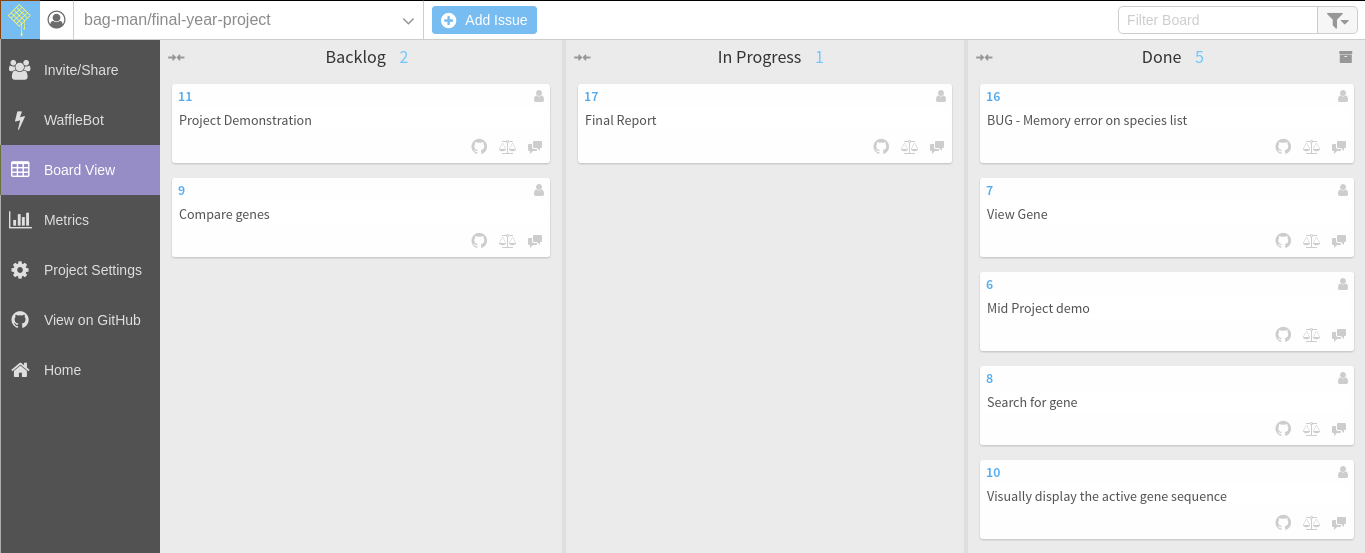
\includegraphics[scale=0.3]{waffle}
\caption{Kanban board in use. Waffle.io is the service providing the board}
\end{center}
\end{figure}

However as this project involved a lot of domain knowledge that wasn't familiar, there was a very significant amount of time spent learning what the data meant and how it should be used. During that time I was prototyping potential solutions to how the data could be interpreted, without a specific set of requirements in mind. This lead to very vague requirements being created and development following a path closely linked to the data and my understanding of it. 

An example of this process was the reverse compliment feature, that didn't appear to be necessary until a couple of weeks before the project deadline. This is exactly why a traditional structured development process like waterfall would not have worked for this project, as new requirements and features were appearing deep into the project, something that i wouldn't have been able to accommodated if I were using a strict waterfall model, where each phase of development is scheduled a head of time.

% You need to describe briefly the life cycle model or research method that you used. You do not need to write about all of the different process models that you are aware of. Focus on the process model or research method that you have used. It is possible that you needed to adapt an existing method to suit your project; clearly identify what you used and how you adapted it for your needs.

% For the research-oriented projects, there needs to be a suitable process for the construction of the software elements that support your work. 
